\documentclass[UKenglish,usenames,dvipsnames,svgnames,table,aspectratio=169,mathserif]{beamer}

\mode<presentation> {

%\usetheme{default}
\usetheme{Madrid}

\setbeamertemplate{footline} % To remove the footer line in all slides uncomment this line

\setbeamertemplate{navigation symbols}{} % To remove the navigation symbols from the bottom of all slides uncomment this line
}

\usepackage{graphicx} % Allows including images
\usepackage{booktabs} % Allows the use of \toprule, \midrule and \bottomrule in tables
\usepackage{hyperref}
%\usepackage{apacite}
\usepackage{babel}
\usepackage{fancyvrb}
\usepackage{color}
\usepackage{alltt}
\usepackage{listings}
\usepackage{framed}
\usepackage{courier}
\usepackage{minted}
\usepackage{epstopdf}
\usepackage{xifthen}
\usepackage[utf8]{inputenc}
\usepackage[T1]{fontenc}
\usepackage{textcomp}
\usepackage{gensymb}
\usepackage{svg}
\usepackage{pdfpages}
\usepackage{isodate}
\usepackage{Haskelllogo}

\hypersetup{colorlinks=false}

\setbeamertemplate{bibliography entry title}{}
\setbeamertemplate{bibliography entry location}{}
\setbeamertemplate{bibliography entry note}{}
\setbeamertemplate{itemize items}[circle]
\setbeamertemplate{enumerate items}[circle]
\beamertemplatenavigationsymbolsempty
\setbeamertemplate{footline}{}


\newminted{haskell}{}

\definecolor{g}{RGB}{0,100,0}
\newcommand{\highlight}[1]{\colorbox{yellow}{#1}}
\newcommand{\nega}[1]{\colorbox{yellow}{#1}}
\newcommand{\posi}[1]{\colorbox{green}{#1}}
\newcommand{\nl}{\vspace{\baselineskip}}
\newcommand{\pnl}{\pause \nl}

\graphicspath{{diagrams/}}

\newcommand{\textslide}[1]{{
\begin{frame}
\begin{center}

#1

\end{center}
\end{frame}
}}

\newcommand{\textslideleft}[1]{{
\begin{frame}

#1

\end{frame}
}}

\newcommand{\codeslide}[1]{{
\begin{frame}[fragile]
\begin{haskellcode}
#1
\end{haskellcode}
\end{frame}
}}


\newcommand{\imageslide}[2][1]{{
\begin{frame}\begin{center}
\includegraphics[scale=#1]{#2}
\end{center}\end{frame}
}}

\newcommand{\imageslideleft}[2][1]{{
\begin{frame}
\includegraphics[scale=#1]{#2}
\end{frame}
}}

\newcommand{\imagetextslide}[3][1]{{
\begin{frame}\begin{center}

{#3}

\includegraphics[scale=#1]{#2}
\end{center}\end{frame}
}}

\newcommand{\svgslide}[1]{{
\begin{frame}
\begin{center}
\includesvg{diagrams/#1}
\end{center}
\end{frame}
}}

\newcommand{\latticeinfoslide}[1]{{
\begin{frame}
\begin{columns}
\column{0.7\textwidth}
\includegraphics[scale=0.65]{#1}
\column{0.3\textwidth}
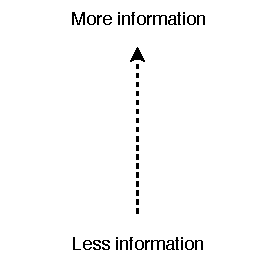
\includegraphics[scale=1.2]{set/more-info.pdf}
\end{columns}
\end{frame}
}}

\definecolor{bgc}{RGB}{255, 255, 255}
\setbeamercolor{background canvas}{bg=bgc}


%%----------------------------------------------------------------------------------------
%	TITLE PAGE
%----------------------------------------------------------------------------------------

\title[Propagators]{An Intuition for Propagators}
\titlegraphic{
\includegraphics[scale=0.25]{data61.png}}
\author{George Wilson}
\institute[]
{
CSIRO's Data61\\
\medskip
\href{george.wilson@data61.csiro.au}{george.wilson@data61.csiro.au}
}

\selectlanguage{UKenglish}
\date{\printdate{2019-09-02}}

\begin{document}

%%%%%
%%%%% Intro section
%%%%%

\begin{frame}
\titlepage
\end{frame}


\begin{frame}

\huge \centering 1970s, MIT
\end{frame}


\begin{frame}

\Large \centering
a model of computation for {\bf highly concurrent} machines
\end{frame}


\imageslide[1.8]{intro-cell0.pdf}
\imageslide[1.8]{intro-cell1.pdf}
\imageslide[1.8]{intro-cell2.pdf}

\imageslide[1.5]{intro-prop0.pdf}
\imageslide[1.5]{intro-prop1.pdf}
\imageslide[1.5]{intro-prop2.pdf}
\imageslide[1.5]{intro-prop3.pdf}
\imageslide[1.5]{intro-prop4.pdf}
\imageslide[1.5]{intro-prop5.pdf}
\imageslide[1.5]{intro-prop6.pdf}


\begin{frame}[fragile]
\begin{haskellcode}
-- types
data Par a
instance Monad Par

data Cell a
\end{haskellcode}
\pnl
\begin{haskellcode}
-- Creating a cell
cell    :: Par (Cell a)
\end{haskellcode}
\pnl
\begin{haskellcode}
-- Working with Cells
content :: Cell a -> Par (Maybe a)
write   :: Cell a -> a -> Par ()
\end{haskellcode}
\pnl
\begin{haskellcode}
-- Creating a propagator
watch   :: Cell a -> (a -> Par ()) -> Par ()
\end{haskellcode}
\end{frame}


\begin{frame}[fragile]
\centering

\begin{columns}
\begin{column}{0.5\textwidth}
\begin{overlayarea}{0.5\textwidth}{0.4\textheight}
\begin{onlyenv}<1>
\includegraphics[scale=0.8]{intro-toUpper0.pdf}
\end{onlyenv}
\begin{onlyenv}<2>
\includegraphics[scale=0.8]{intro-toUpper1.pdf}
\end{onlyenv}
\begin{onlyenv}<3>
\includegraphics[scale=0.8]{intro-toUpper2.pdf}
\end{onlyenv}
\begin{onlyenv}<4>
\includegraphics[scale=0.8]{intro-toUpper3.pdf}
\end{onlyenv}
\begin{onlyenv}<5->
\includegraphics[scale=0.8]{intro-toUpper4.pdf}
\end{onlyenv}
\end{overlayarea}
\end{column}
\begin{column}{0.5\textwidth}
\begin{overlayarea}{\textwidth}{0.5\textheight}
\begin{onlyenv}<1->
\begin{haskellcode}
do
  input  <- cell
\end{haskellcode}
\end{onlyenv}
\begin{onlyenv}<2->
\begin{haskellcode}
  output <- cell
\end{haskellcode}
\end{onlyenv}
\begin{onlyenv}<3-5>
\begin{minted}{haskell}
  watch input (\c ->
    write output (toUpper c))
\end{minted}
\end{onlyenv}
\begin{onlyenv}<6>
\begin{minted}[highlightlines={1,2}]{haskell}
  watch input (\c ->
    write output (toUpper c))
\end{minted}
\end{onlyenv}

\nl
\begin{onlyenv}<4->
\begin{haskellcode}
  write input 'q'
  content output   -- Just 'Q'
\end{haskellcode}
\end{onlyenv}
\end{overlayarea}
\end{column}
\end{columns}
\end{frame}


\begin{frame}[fragile]
\begin{haskellcode}
          lift :: (a -> b) -> Cell a -> Cell b -> Par ()
          lift f input output =
            watch input (\a ->
              write output (f a))
\end{haskellcode}
\end{frame}


\begin{frame}[fragile]
\centering

\begin{columns}
\begin{column}{0.5\textwidth}
\begin{overlayarea}{0.5\textwidth}{0.4\textheight}
\includegraphics[scale=0.8]{intro-toUpper4.pdf}
\end{overlayarea}
\end{column}
\begin{column}{0.5\textwidth}
\begin{haskellcode}
do
  input  <- cell
\end{haskellcode}
\begin{haskellcode}
  output <- cell
\end{haskellcode}
\begin{minted}[highlightlines=1]{haskell}
  lift toUpper input output
\end{minted}
\nl
\begin{haskellcode}
  write input 'q'
  content output   -- Just 'Q'
\end{haskellcode}
\end{column}
\end{columns}

\end{frame}


\begin{frame}[fragile]
\centering


\begin{columns}
\begin{column}{0.5\textwidth}
\begin{overlayarea}{0.5\textwidth}{0.4\textheight}
\begin{onlyenv}<1>
\includegraphics[scale=0.9]{build-adder0.pdf}
\end{onlyenv}
\begin{onlyenv}<2->
\includegraphics[scale=0.9]{build-adder1.pdf}
\end{onlyenv}
\end{overlayarea}
\end{column}
\begin{column}{0.5\textwidth}
\begin{haskellcode}
do
  inL  <- cell
  inR  <- cell
  out  <- cell
\end{haskellcode}
\pnl
\begin{haskellcode}
  watch inL (\x -> do
    maybeY <- content inR
    case maybeY of
      Nothing -> pure ()
      Just y  -> write out (x+y)
\end{haskellcode}
\pnl
\begin{haskellcode}
  watch inR (\y -> do
    maybeX <- content inL
    case maybeX of
      Nothing -> pure ()
      Just x  -> write out (x+y)
\end{haskellcode}
\end{column}
\end{columns}
\end{frame}


\begin{frame}[fragile]
\begin{haskellcode}
          with :: Cell a -> (a -> Par ()) -> Par ()
          with theCell callback = do
            maybeA <- content theCell
              case maybeA of
                Nothing -> pure ()
                Just a  -> callback a
\end{haskellcode}
\end{frame}


\begin{frame}[fragile]
\centering

\begin{columns}
\begin{column}{0.5\textwidth}
\begin{overlayarea}{0.5\textwidth}{0.4\textheight}
\includegraphics[scale=0.8]{build-adder1.pdf}
\end{overlayarea}
\end{column}
\begin{column}{0.5\textwidth}
\begin{haskellcode}
do
  inL  <- cell
  inR  <- cell
  out  <- cell
\end{haskellcode}
\nl
\begin{haskellcode}
  watch inL (\x ->
    with inR (\y ->
      write out (x+y)
\end{haskellcode}
\pnl
\begin{haskellcode}
  watch inR (\y ->
    with inL (\x ->
      write out (x+y)
\end{haskellcode}
\end{column}
\end{columns}
\end{frame}


\begin{frame}[fragile]
\begin{haskellcode}
          lift2 :: (a -> b -> c)
                -> Cell a -> Cell b -> Cell c
                -> Par ()
\end{haskellcode}
\pause
\begin{haskellcode}
          lift2 f inL inR out = do
            watch inL (\a ->
              with inR (\b ->
                write out (f a b)))
            watch inR (\b ->
              with inL (\a ->
                write out (f a b)))
\end{haskellcode}

\end{frame}


\begin{frame}[fragile]
\centering

\begin{columns}
\begin{column}{0.5\textwidth}
\begin{overlayarea}{0.5\textwidth}{0.4\textheight}
\includegraphics[scale=0.8]{build-adder1.pdf}
\end{overlayarea}
\end{column}
\begin{column}{0.5\textwidth}
\begin{haskellcode}
do
  inL  <- cell
  inR  <- cell
  out  <- cell
\end{haskellcode}
\nl
\begin{haskellcode}
  adder inL inR out

    where
      adder l r o = do
        lift2 (+) l r o
        lift2 (-) o l r
        lift2 (-) o r l
\end{haskellcode}
\end{column}
\end{columns}
\end{frame}


\imageslide{oscillator0.pdf}
\imageslide{oscillator1.pdf}
\imageslide{oscillator2.pdf}
\imageslide{oscillator3.pdf}
\imageslide{oscillator4.pdf}
\imageslide{oscillator5.pdf}
\imageslide{oscillator6.pdf}
\imageslide{oscillator7.pdf}
\imageslide{oscillator8.pdf}


\begin{frame}
\centering
\fontsize{60}{70}\selectfont $?!$

\end{frame}


\begin{frame}
\centering \huge

How can we fix this?
\end{frame}


\begin{frame}[fragile]
\begin{columns}
\column{0.1\textwidth}
\column{0.7\textwidth}
\begin{overlayarea}{\textwidth}{0.6\textheight}
\begin{haskellcode}
data WriteOnce a
  = None
  | Written a
  | TooMany
\end{haskellcode}

\nl

\begin{onlyenv}<2>
\begin{haskellcode}
tryWrite ::           a -> WriteOnce a -> WriteOnce a
tryWrite a w = case w of
  None      -> Written a
  Written b -> TooMany
  TooMany   -> TooMany
\end{haskellcode}
\end{onlyenv}

\begin{onlyenv}<3->
\begin{haskellcode}
tryWrite :: (Eq a) => a -> WriteOnce a -> WriteOnce a
tryWrite a w = case w of
  None      -> Written a
  Written b -> if a == b then Written b else TooMany
  TooMany   -> TooMany
\end{haskellcode}
\end{onlyenv}
\end{overlayarea}
\column{0.2\textwidth}
\end{columns}
\end{frame}


\imageslide{oscillator-fixed1.pdf}
\imageslide{oscillator-fixed2.pdf}
\imageslide{oscillator-fixed3.pdf}
\imageslide{oscillator-fixed4.pdf}
\imageslide{oscillator-fixed5.pdf}
\imageslide{oscillator-fixed6.pdf}
\imageslide{oscillator-fixed7.pdf}


\begin{frame}

\centering \LARGE

Mutability is {\bf chaos}

\nl
WriteOnce is {\bf rigid}
\end{frame}


\begin{frame}[fragile]

\LARGE
\begin{center}
Accumulate information about a value

\pnl

{\bf monotonically}
\end{center}
\end{frame}


% \begin{frame}
% \Large

% Now every network will give a
% {\bf deterministic answer}
% in {\bf finite time}
% \end{frame}


\begin{frame}[fragile]

\begin{haskellcode}
data WriteOnce a

  -- I have heard contradictory answers!
  = TooMany

  -- I know the answer exactly
  | Written a

  -- I don't know anything
  | None
\end{haskellcode}

% \pnl

% \centering \Large
% {\bf Monotonic} growth

\end{frame}


% \begin{frame}[fragile]

% \begin{overlayarea}{\textwidth}{0.6\textheight}

% \begin{minted}{haskell}
% mergeWrites :: WriteOnce a -> WriteOnce a -> WriteOnce a
% \end{minted}
% \begin{onlyenv}<1>
% \begin{minted}[highlightlines={}]{haskell}
% mergeWrites  a            None       = a
% mergeWrites  None         b          = b
% mergeWrites  TooMany      b          = TooMany
% mergeWrites  a            TooMany    = TooMany
% mergeWrites (Written a)  (Written b) = 
%     if a == b then Written a else TooMany
% \end{minted}
% \end{onlyenv}
% \begin{onlyenv}<2>
% \begin{minted}[highlightlines={1,2}]{haskell}
% mergeWrites  a            None       = a
% mergeWrites  None         b          = b
% mergeWrites  TooMany      b          = TooMany
% mergeWrites  a            TooMany    = TooMany
% mergeWrites (Written a)  (Written b) = 
%     if a == b then Written a else TooMany
% \end{minted}
% \end{onlyenv}
% \begin{onlyenv}<3>
% \begin{minted}[highlightlines={3,4}]{haskell}
% mergeWrites  a            None       = a
% mergeWrites  None         b          = b
% mergeWrites  TooMany      b          = TooMany
% mergeWrites  a            TooMany    = TooMany
% mergeWrites (Written a)  (Written b) = 
%     if a == b then Written a else TooMany
% \end{minted}
% \end{onlyenv}
% \begin{onlyenv}<4>
% \begin{minted}[highlightlines={5,6}]{haskell}
% mergeWrites  a            None       = a
% mergeWrites  None         b          = b
% mergeWrites  TooMany      b          = TooMany
% mergeWrites  a            TooMany    = TooMany
% mergeWrites (Written a)  (Written b) = 
%     if a == b then Written a else TooMany
% \end{minted}
% \end{onlyenv}
% \end{overlayarea}
% \end{frame}


\imageslide[0.6]{sudoku/sudoku1.png}
\imageslide[0.6]{sudoku/sudoku2.png}
\imageslide[0.6]{sudoku/sudoku3.png}
\imageslide[0.6]{sudoku/sudoku4.png}
\imageslide[0.6]{sudoku/sudoku5.png}
\imageslide[0.6]{sudoku/sudoku6.png}
\imageslide[0.6]{sudoku/sudoku7.png}
\imageslide[0.6]{sudoku/sudoku8.png}
\imageslide[0.6]{sudoku/sudoku9.png}
\imageslide[0.6]{sudoku/sudoku10.png}
\imageslide[0.6]{sudoku/sudoku11.png}
\imageslide[0.6]{sudoku/sudoku12.png}
\imageslide[0.6]{sudoku/sudoku13.png}


\begin{frame}
\begin{columns}
\column{0.7\textwidth}
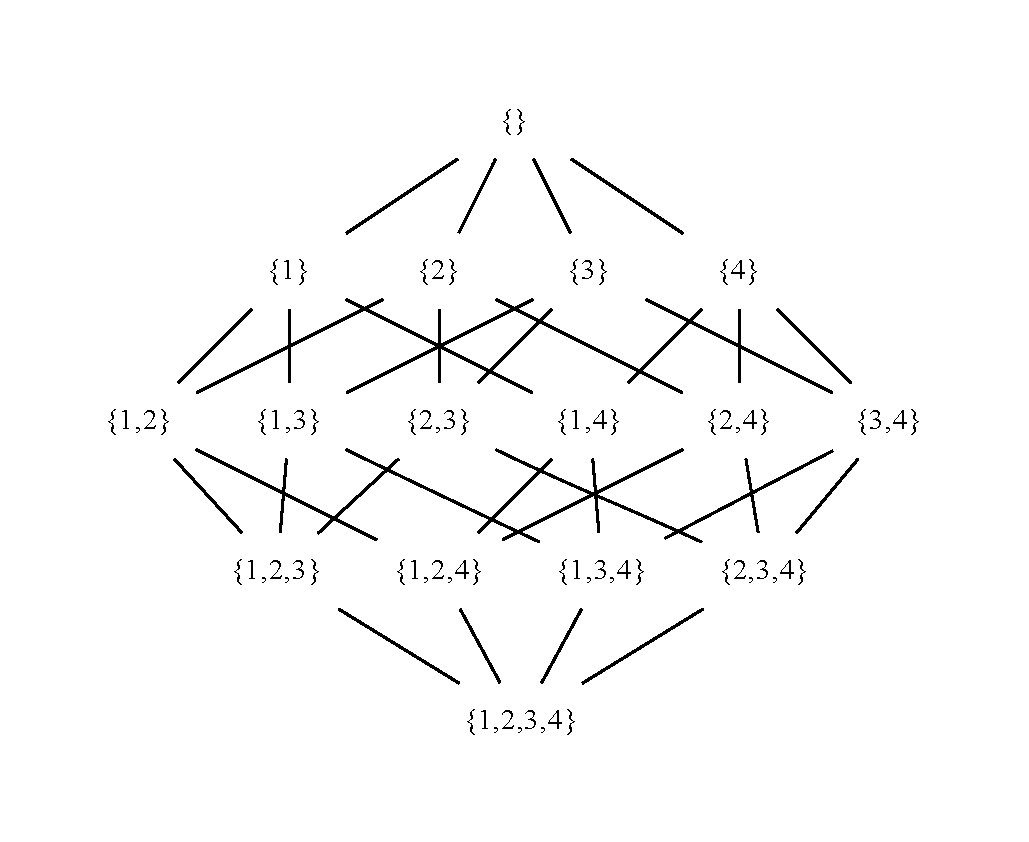
\includegraphics[scale=0.65]{set/powerset.pdf}
\pause
\column{0.3\textwidth}
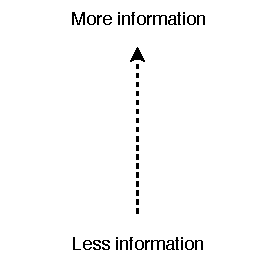
\includegraphics[scale=1.2]{set/more-info.pdf}
\end{columns}
\end{frame}


\latticeinfoslide{set/powerset-info1.pdf}
\latticeinfoslide{set/powerset-info2.pdf}
\latticeinfoslide{set/powerset-info3.pdf}
\latticeinfoslide{set/powerset-info4.pdf}

\latticeinfoslide{set/powerset1.pdf}
\latticeinfoslide{set/powerset2.pdf}
\latticeinfoslide{set/powerset3.pdf}
\latticeinfoslide{set/powerset4.pdf}
\latticeinfoslide{set/powerset5.pdf}
\latticeinfoslide{set/powerset6.pdf}


% \begin{frame}

% The accumulation must:

% \begin{itemize}
% \item tolerate {\bf reordering} of information
% \item tolerate {\bf grouping} of information
% \item ignore {\bf redundancy} of information
% \end{itemize}
% \end{frame}

% \begin{frame}

% To be deterministic we must

% \begin{itemize}
% \item tolerate {\bf reordering} of writes
% \item tolerate {\bf grouping} of writes
% \item ignore {\bf redundancy} of writes
% \end{itemize}
% \end{frame}


\begin{frame}[fragile]
\centering \huge
Bounded join semilattice
\nl
\large

Identity: \\
$x \vee bottom = bottom = bottom \vee x$
\nl

Associative: \\
$x \vee (y \vee z) = (x \vee y) \vee z$
\nl

Commutative: \\
$x \vee y = y \vee x$
\nl

Idempotent: \\
$x \vee x = x$

\end{frame}


\begin{frame}[fragile]

\begin{overlayarea}{\textwidth}{0.5\textheight}
\begin{haskellcode}
class SemiLattice a where
  (\/)   :: a -> a -> a
  bottom :: a
\end{haskellcode}
\nl

\begin{onlyenv}<2>
\begin{haskellcode}
instance (Eq a) => SemiLattice (WriteOnce a) where
  None      \/ b           = b
  TooMany   \/ x           = TooMany
  Written a \/ None        = Written a
  Written a \/ TooMany     = TooMany
  Written a \/ Written b   = if a == b then Written a else TooMany
\end{haskellcode}
\end{onlyenv}
\begin{onlyenv}<3>
\begin{haskellcode}
data SudokuVal = One | Two | Three | Four deriving (Eq, Ord)

data Possibilities = Pos (Set SudokuVal)

instance Semilattice Possibilities where
  Pos p \/ Pos q = Pos (Set.intersection p q)
  bottom = Pos (Set.fromList [One,Two,Three,Four])
\end{haskellcode}
\end{onlyenv}
\end{overlayarea}
\end{frame}


\begin{frame}
\begin{columns}
\column{0.7\textwidth}
\includegraphics{writeonce-bool0.pdf}
\column{0.3\textwidth}
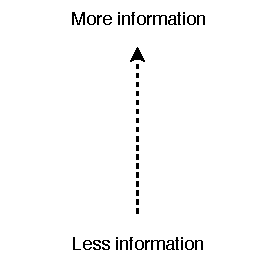
\includegraphics[scale=1.3]{set/more-info.pdf}
\end{columns}
\end{frame}


\begin{frame}
\LARGE \centering

Cells hold semilattices

Propagators always join information in
\end{frame}


\begin{frame}

\centering
WriteOnce (aka IVar, Promise) \\
Sets (intersection or union) \\
Intervals \\
Search \\
many many more
\end{frame}


% \begin{frame}

% \centering \huge
% Monotonicity
% \nl

% \Large
% $f$ is monotone if\\
% \nl

% $ x \leq y \implies f(x) \leq f(y)$

% \end{frame}


\begin{frame}
\huge \centering
Thanks for listening!
\nl

\large
(Real) code for all these examples and more:

\url{https://github.com/qfpl/propagator-examples}

\end{frame}


\end{document}
